\chapter{Asking Miami Millionaires How They Got Rich}

This chapter follows a School of Hard Knocks interview, curated by LazyingArt LLC, and it is best read as a lecture in operational mathematics rather than symbolic mathematics. We are not given a single formula for wealth. Instead, we are taken through a sequence of local rules: save first, scale in stages, invest where there is traction, learn by failing faster, recruit talent through leadership and product strength, and avoid the distortions created by comparison. The transcript is informal, but its underlying structure is disciplined enough that we can write it as a chain of definitions, inequalities, and causal dependencies.

\section{Miami as a Sampling Device for Wealth Paths}

We begin with a repeated question: what would one tell a younger self starting from zero? The repetition is not accidental. It turns Miami into a sampling device. Social media marketing, commercial real estate, professional sport, and competitive intelligence appear side by side, and the diversity of the answers already tells us something important: wealth is not confined to one privileged domain.

The first lesson of the lecture is therefore negative. There is no single industry's theorem of success here. The positive lesson comes only after the montage slows down: across these different careers, the same mechanisms reappear. We hear about saving discipline, modeled behavior, market assessment, traction, recruiting, product quality, and the surrounding environment. The lecture begins with breadth so that it can later earn its abstractions.

This opening montage also fixes the lecture's baseline condition. Nearly every useful answer is framed against the same initial state: starting from zero. The notes should preserve that baseline, because it is what turns scattered anecdotes into rules that claim generality.

\section{Savings Discipline and the First Structure of Scale}

The first extended framework comes from a speaker who reports a four-million-dollar year, places himself in business development and sales, and then begins with a rule so simple that it might look trivial if we do not listen carefully enough. He is told to place a fixed portion of income into a stock index fund and to treat the rest of his investing life as something separate. In the notes we may express that compactly as
\begin{equation}
I_{\mathrm{idx}} = 0.10\,Y,
\end{equation}
where $Y$ is income and $I_{\mathrm{idx}}$ is the protected index allocation.

This matters because the lecture does not present the rule as a complete portfolio theory. It presents it as a floor: one part of wealth-building is to establish a non-negotiable bucket that is not continually revised by mood, vanity, or market chatter. The insistence to ``follow that strictly'' is the substantive part.

From there the lecture immediately pivots to scale. This is the first point where the narration moves from personal finance to a more structural picture of growth. We are told that scaling does not happen on one unbroken line. It comes in levels, or tranches, and the next level may not resemble the previous one at all. A concise notation for the lecture's picture is
\begin{equation}
G=\{G_1,G_2,G_3\},
\end{equation}
where $G_1$ is the initial phase of blood, sweat, and tears, and $G_2,G_3$ stand for later stages whose requirements differ from the first and from each other.

The force of the claim lies in the asymmetry between stages. A first great jump can be powered by founder effort, improvisation, and direct contact with the market. A later jump cannot simply repeat that same recipe at a larger scale. The second hundred million is not produced by the same machine that produced the third. That is why the lecture introduces stages before it introduces technique.

\subsection{Question \& Answer}

The lecture then asks a sharply focused question: how do we get from a seven-figure business to an eight-figure business? This question should survive in the chapter as a distinct block because it marks the moment when the lecture stops admiring scale and starts analyzing its preconditions.

\begin{proposition}
A first million is not, by itself, evidence that an eight-figure path exists.
\end{proposition}

\begin{proof}
The lecture supplies at least three alternative explanations for an early win: luck, support from friends and family, or a good idea that is simply not scalable. None of these explanations guarantees that the business sits inside a sufficiently large market. Therefore the next question is not merely whether one can work harder. The next question is whether the addressable market is large enough and whether the next tranche requires a different operating model.
\end{proof}

We may summarize the decision rule as
\begin{equation}
\text{8-figure scale} \Rightarrow M_{\mathrm{addr}} \text{ is sufficiently large},
\end{equation}
where $M_{\mathrm{addr}}$ is the effective addressable market, the safest formal gloss for what the speaker calls the ``green field.''

The lecture's answer is then sequential. First, diagnose whether the initial success was structural or accidental. Second, ask what headroom the market actually provides. Third, if the market is real, choose the right path to enter it. Fourth, do not attempt that diagnosis alone. Experts matter here not as prestige, but as measurement devices. They keep us from mistaking an exciting first result for a scalable business.

\section{Competitive Intelligence, Retirement, and Traction}

After a brief comic reset, the lecture pivots to a speaker who calls himself a spymaster. The term is playful, but the underlying definition is sober.

\begin{definition}
\emph{Competitive intelligence} is the disciplined monitoring of a company's external environment, in an analogous way to how a government watches for external and internal threats.
\end{definition}

This definition is not decorative. It prepares the next moves. If one's job is to watch the environment before acting, then the relevant financial advice is not speculative heroism but disciplined self-protection: pay yourself first, push money toward retirement, and do not assume that public systems will carry the full burden later.

The next step is then an investment filter. The lecture advises us not to chase whatever happens to be visible, loud, or fashionable. We are instead told to look for traction and to invest there.

\begin{definition}
\emph{Traction} is observable evidence that demand is real and that the company is not merely a temporary or ``fly-by-night'' construction.
\end{definition}

This is a small but important structural point. Attention comes before allocation. We first read the field; only then do we commit capital. In that sense the lecture aligns intelligence work with investing: the discipline is not to move first, but to see first.

The same speaker then broadens the register. The usual slogan ``you only live once'' is revised into a more interesting asymmetry: one dies once, but one lives every day. In the argument of the chapter, this is not merely motivational garnish. It preserves a rhythm the lecture cares about. The same person who says ``pay yourself first'' also says that one should not postpone life until some abstract future. Financial structure and existential tempo are made to coexist.

\section{Miami as a Multiplier and Failure as a Method}

The penthouse interview marks a real shift in the lecture. We no longer have a quick street answer. We have a staged environment, a slower pace, and a speaker who explicitly interprets Miami as part of the mechanism. The city is described as a place that does not shame work, that puts visible wealth in ordinary circulation, and that enlarges the perceived size of the game. This is why the scene change matters narratively. The lecture is no longer gathering rules only from biographies; it is now analyzing the surroundings that amplify or suppress ambition.

The speaker's first major principle is that one should fail faster and stop attaching excessive meaning to small failures. The notes should not flatten this into a slogan. The point is methodological: a failure that is stripped of false significance becomes usable information. A failure treated as identity becomes paralysis.

We can write the implicit logic in a deliberately modest way:
\begin{align}
\text{smaller emotional penalty} &\Rightarrow \text{faster iteration},\\
\text{faster iteration} &\Rightarrow \text{more learning per unit time},\\
\text{more learning per unit time} &\Rightarrow \text{greater compounded adaptation}.
\end{align}
This is not a theorem spoken in symbolic form by the interviewee, but it is the cleanest cautious reconstruction of the argument.

\subsection{Question \& Answer}

The lecture then asks a direct explanatory question: why do some ecosystems produce more billion-dollar startups? The speaker answers by invoking Israel as a case of accelerated learning, where failure is treated not as terminal shame but as part of intelligent forward motion.

The structure of the answer is worth preserving. The claim is not simply that successful ecosystems are ``ambitious.'' The stronger claim is that they remove false significance from mistakes, shorten the loop between action and correction, and let time compound learning. The lecture's causal line is therefore
\begin{enumerate}
\item fail without theatrical self-destruction,
\item extract the lesson quickly,
\item shorten the interval before the next attempt,
\item let those shortened cycles accumulate.
\end{enumerate}

What matters in the notes is not the exact statistical force of the Israel example, which the transcript states rhetorically rather than formally. What matters is the mechanism: ecosystems outperform when they make iteration cheap in psychic terms and therefore frequent in practical terms.

\section{The Dependency Chain of Scale}

The penthouse segment then turns into the most explicitly structured argument of the lecture. The speaker cites Ryan Breslow as an object of study and names fundraising and recruiting as the two big lessons. But as the explanation unfolds, those terms are not left standing alone. They are embedded in a longer dependency chain.

\begin{remark}
The chain below is an editorial reconstruction of the lecture's logic. It is not a board derivation, and it should be read as a compact organization of the speaker's sequence rather than as a formally proved theorem.
\end{remark}

The transcript supports the following relations:
\begin{align}
Q &\Rightarrow V \Rightarrow L,\\
L &\Rightarrow R,\\
F &\Rightarrow K \Rightarrow \text{scale},\\
Q &\Rightarrow C \Rightarrow T.
\end{align}
Here $Q$ is product quality, $V$ visionary clarity, $L$ leadership, $R$ recruiting capacity, $F$ fundraising, $K$ deployable cash, $C$ compensation capacity, and $T$ top-tier talent.

The lecture does not state these arrows all at once. It arrives at them verbally. First, cash is needed to scale. Next, leadership is needed to scale and hire. Next, leadership depends on vision. Next, vision depends on product. Finally, talent depends not only on aspiration but on compensation, and compensation in turn depends on the strength of the underlying product. The argument is not perfectly linear, but it is unmistakably hierarchical.

We may schematize the lecture's chain as follows.

\begin{figure}
\centering
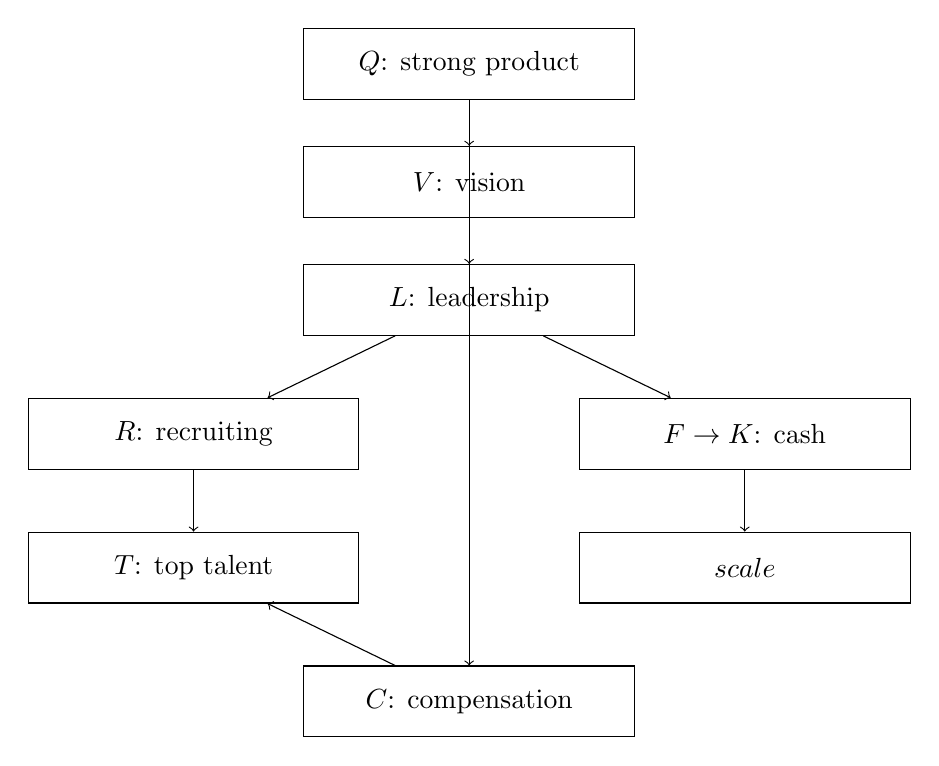
\begin{tikzpicture}
\node[draw, rectangle, minimum width=4.2cm, minimum height=0.9cm] (q) at (0,0) {$Q$: strong product};
\node[draw, rectangle, minimum width=4.2cm, minimum height=0.9cm] (v) at (0,-1.5) {$V$: vision};
\node[draw, rectangle, minimum width=4.2cm, minimum height=0.9cm] (l) at (0,-3.0) {$L$: leadership};
\node[draw, rectangle, minimum width=4.2cm, minimum height=0.9cm] (r) at (-3.5,-4.7) {$R$: recruiting};
\node[draw, rectangle, minimum width=4.2cm, minimum height=0.9cm] (f) at (3.5,-4.7) {$F \rightarrow K$: cash};
\node[draw, rectangle, minimum width=4.2cm, minimum height=0.9cm] (t) at (-3.5,-6.4) {$T$: top talent};
\node[draw, rectangle, minimum width=4.2cm, minimum height=0.9cm] (s) at (3.5,-6.4) {$\text{scale}$};
\node[draw, rectangle, minimum width=4.2cm, minimum height=0.9cm] (c) at (0,-8.1) {$C$: compensation};

\draw[->] (q) -- (v);
\draw[->] (v) -- (l);
\draw[->] (l) -- (r);
\draw[->] (l) -- (f);
\draw[->] (r) -- (t);
\draw[->] (f) -- (s);
\draw[->] (q) -- (c);
\draw[->] (c) -- (t);
\end{tikzpicture}
\end{figure}

This is also the point where the lecture distinguishes industries. In e-commerce, one can imagine a strong product, one platform, and a scaling ad engine. In finance, private equity, and technology, the emphasis shifts: top-tier talent becomes the scarce variable. The lecture is careful not to deny product. It says rather that, in talent-intensive fields, product strength alone is not enough; one must build the cash and compensation structures that can attract exceptional people.

\section{Brickell: Relationships, Credit, and Institutional Work}

The lecture then returns to the street and re-enters a more modular mode. A software engineer says he works for himself, builds apps for Penn State University, Lockheed Martin, and the state of Texas, and reports a two-million-dollar year. The content here is useful because it ties technical labor to institutional trust. The career is not framed as freelancing in the abstract; it is framed as repeatedly becoming legible to serious clients.

The next rule is that relationships are everything. But the lecture does not leave this as networking sentiment. It sharpens the point: when one sits down with somebody, one should come with something to offer. We may therefore define the operative object as relationship capital, not mere proximity.

The same speaker then gives a different savings heuristic:
\begin{equation}
s=0.70,\qquad c=0.30,\qquad s+c=1.
\end{equation}
Here $s$ is the saving share of income and $c$ is the operating or spending share. The lecture also places this rule next to a recommendation to leverage credit so as to preserve cash.

\paragraph{Worked Example.}
The lecture itself gives a two-million-dollar annual income in this segment. If we use that figure only as an illustrative arithmetic input, then the 70/30 rule yields
\begin{align}
sY &= 0.70Y = \$1{,}400{,}000,\\
cY &= 0.30Y = \$600{,}000.
\end{align}
By comparison, the earlier index-fund rule would isolate
\begin{equation}
I_{\mathrm{idx}} = 0.10Y = \$200{,}000.
\end{equation}
The chapter should state explicitly that these are different speaker-specific heuristics, not a unified doctrine announced by the lecture itself.

What is common between them is not the exact percentage. What is common is the insistence that income must be partitioned by rule before it is consumed by noise. That is the real mathematical habit the lecture keeps rediscovering.

\section{Brand, Product, Place, and Psychological Discipline}

The next speaker recounts a path from social media marketing to owned e-commerce brands. The turning point is revealing: he grows tired of client work, notices that running a business can still leave one under the command of other people, and then moves from servicing brands to building them. This is the lecture's shift from agency economics to asset economics.

His account of brand is deliberately vivid. A true brand changes the structure of a customer's response. One no longer asks why one should jump. One asks only how high. Apple is used as the canonical example: the lecture's point is not a careful revenue decomposition of AirPods, but the more general fact that a powerful brand lowers the friction of demand across product lines.

The e-commerce advice is then stated with unusual clarity:
\begin{equation}
Q \succ Mkt \succ Sal,
\end{equation}
where $Q$ stands for product quality, $Mkt$ for marketing, and $Sal$ for sales. The lecture immediately adds two asymmetries:
\begin{align}
Q \uparrow &\Rightarrow \text{need}(Mkt)\downarrow,\\
Mkt \uparrow &\Rightarrow \text{need}(Sal)\downarrow.
\end{align}
The point is not that marketing or sales disappear, but that a strong product changes the burden borne by the later layers.

This same stretch of the lecture also returns to Miami as a force multiplier. One speaker says the city makes him want to level up, to work harder, to preserve a base elsewhere but come to Miami when he wants to work in a place that feels almost unreal. Another speaker, a professional soccer player, translates success into the ability to carry pressure, even the pressure of carrying family expectations. These remarks are not separate from the earlier sections. They restate the same motif: surrounding conditions affect the scale of action we consider normal.

The commercial real-estate sequence then gives us one of the lecture's cleanest examples of spatial reasoning. A building is chosen because it sits between I-95 and the Florida Turnpike, with the result that a portfolio of properties remains within practical reach:
\begin{equation}
\forall i,\qquad t_i \le 3\,\mathrm{h}.
\end{equation}
This is not geometry for its own sake. It is a reminder that operational range is a business variable.

The Celsius story pushes the logic further. Ownership of an office building is not merely rental income; it is adjacency to people, firms, and latent opportunities. In a compact form the lecture's causal chain is
\begin{equation}
O_{\mathrm{office}} \Rightarrow \text{tenant contact} \Rightarrow \text{acquisition opportunity} \Rightarrow \text{equity upside}.
\end{equation}
The important lesson is not that every office building hides a future public company. It is that positioning changes the set of opportunities one can even see.

The final warning of the lecture is psychological rather than financial, but it too admits a compact structure:
\begin{equation}
\text{comparison} \Rightarrow \text{insecurity} \Rightarrow \text{distorted spending}.
\end{equation}
Many public displays of wealth are fake or at least misleading; comparison encourages people to buy what they cannot afford and to mistake spectacle for progress. The lecture closes by telling us to worry about ourselves, move at our own pace, and refuse the false game of keeping up with appearances. The financial rule and the psychological rule are the same rule seen from two sides: do not let external noise dictate internal allocation.

\section{Summary}

The lecture begins by scattering many careers across the page and ends by revealing that the same mechanisms keep returning. Save first. Treat scale as staged. Do not mistake an early win for a scalable market. Watch for traction before investing. Let failure become information rather than identity. Build product before amplifying it. Understand that talent requires compensation, compensation requires economic strength, and environment affects the size of the ambitions we consider natural.

What makes the transcript useful is precisely that it is not a single polished doctrine. It is a succession of field observations from people who arrived at wealth by different routes. The chapter's job is not to invent a false unity, but to extract the small mathematics already latent in the talk: partitions of income, staged growth, priority orderings, dependency chains, spatial constraints, and behavioral feedback loops. Those are the lecture's durable objects.